\subsection*{True extrapolation fails under both conditioning schemes}

The frozen training boundary was $-4.084499111$ in $\log_{10}(\mathrm{S\,cm^{-1}})$, with 4,819 rows at or below full-source Q80. We evaluated Q90, Q100, and targets at the training maximum plus 0.25 and 0.50 log units. The benchmark used continuous conditioning, the fixed-threshold binary negative control and an unconditional reranking arm, with five matched seeds and the same 1,000-step, temperature-1.0, top-k-40 protocol.

The decisive metric was \emph{frontier-crossing predicted hit rate}: the fraction of candidates that passed validity, novelty, support and uncertainty gates and whose independent RF prediction crossed the frozen training boundary in the requested direction. This rate was 0.0 for continuous conditioning at all four queries and 0.0 for binary conditioning at all four queries. For continuous conditioning, validity fell from 0.564 at Q90 to 0.280 at Q100; at train-max+0.50, validity was 0.390 and target MAE was 0.718, but the mean RF prediction remained near $-4.30$, below the training frontier.

\begin{figure}[H]
\centering
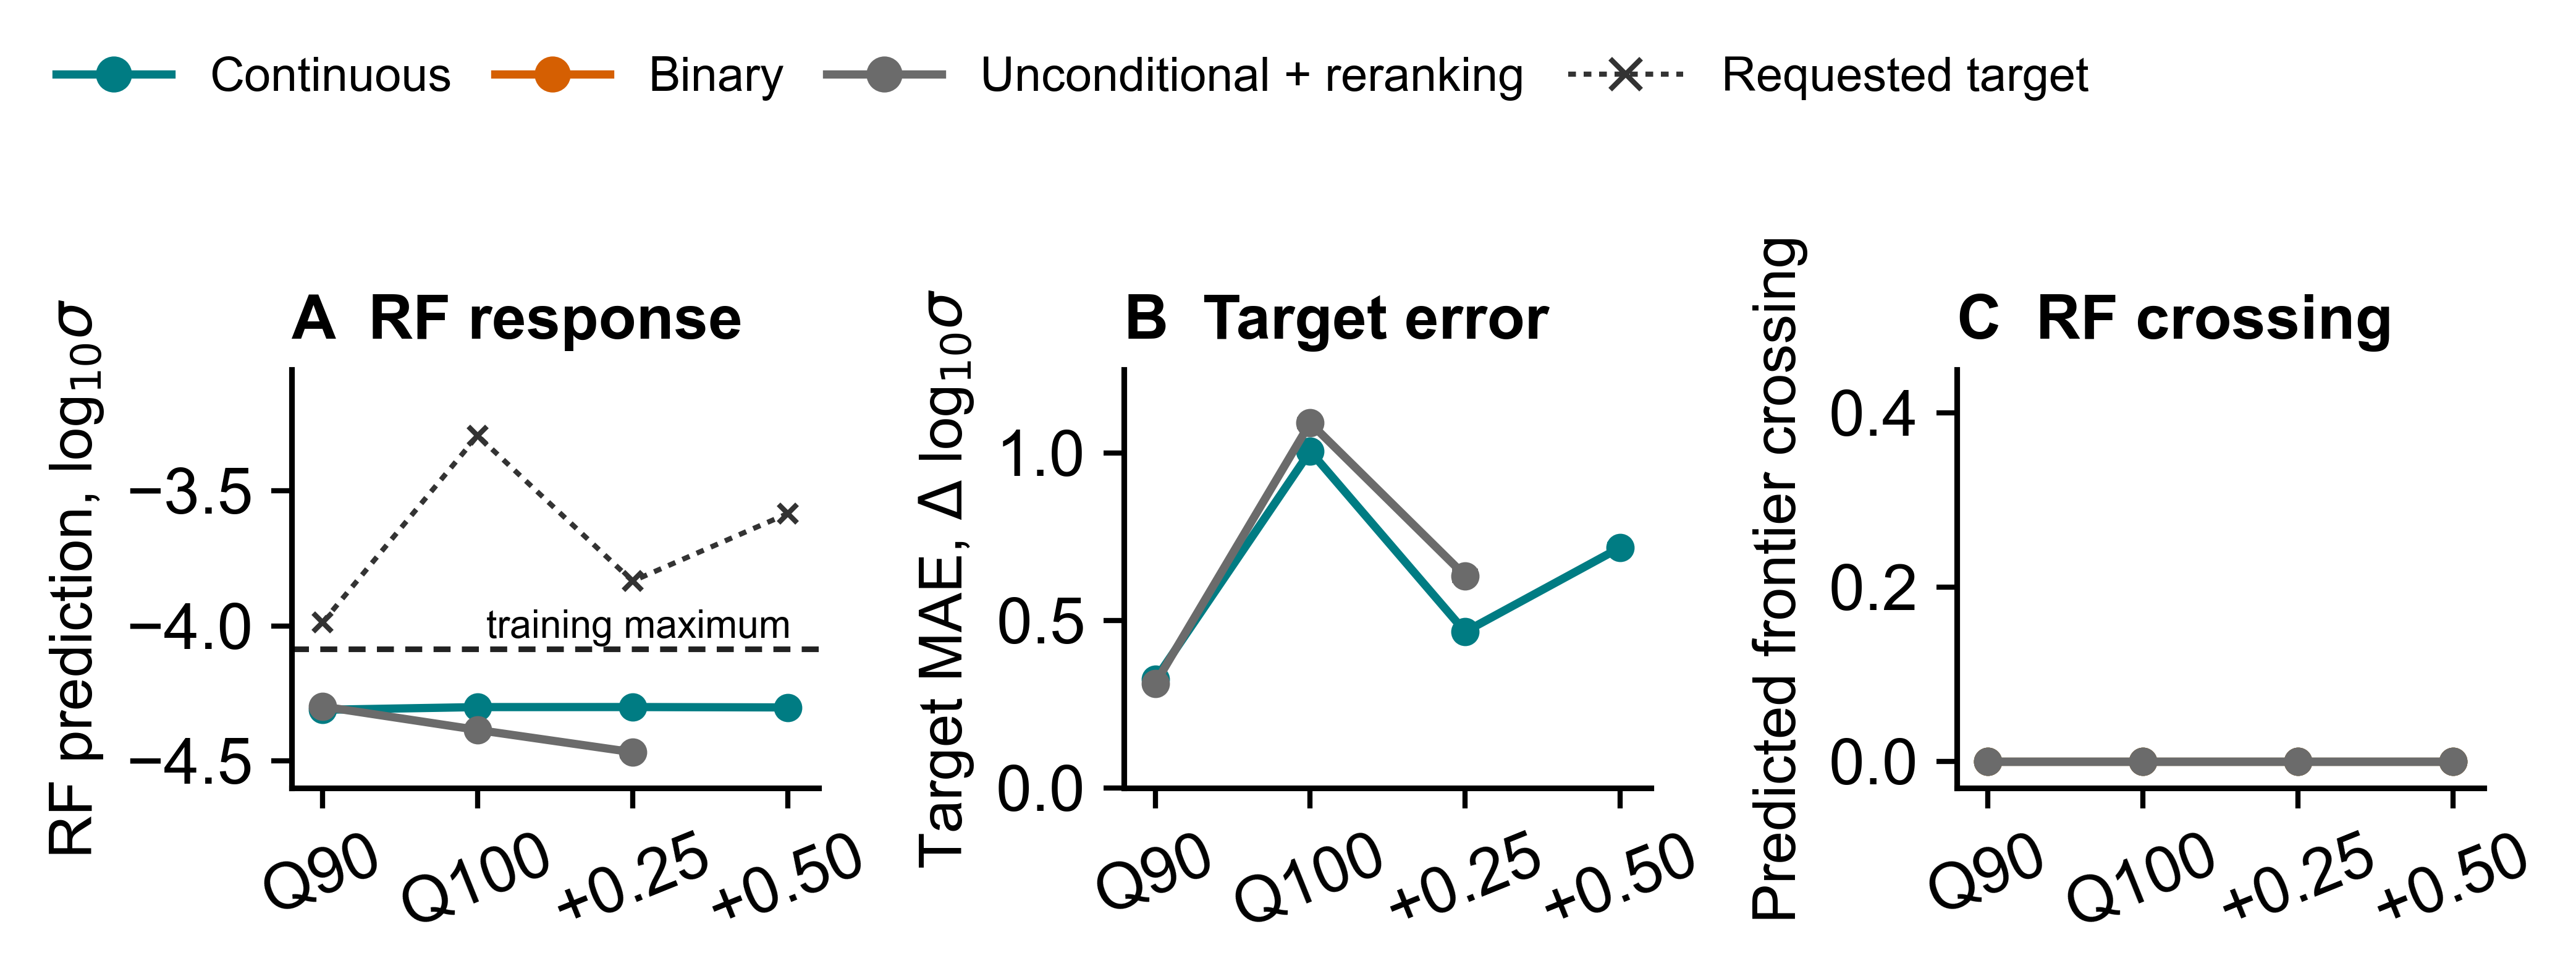
\includegraphics[width=0.98\linewidth]{figures/Figure_1_extrapolation_response.png}
\caption{True extrapolation response. Requested targets move beyond the frozen training support, but RF-predicted candidates do not cross the training frontier for either continuous or binary conditioning.}
\label{fig:extrapolation-response}
\end{figure}

\begin{figure}[H]
\centering
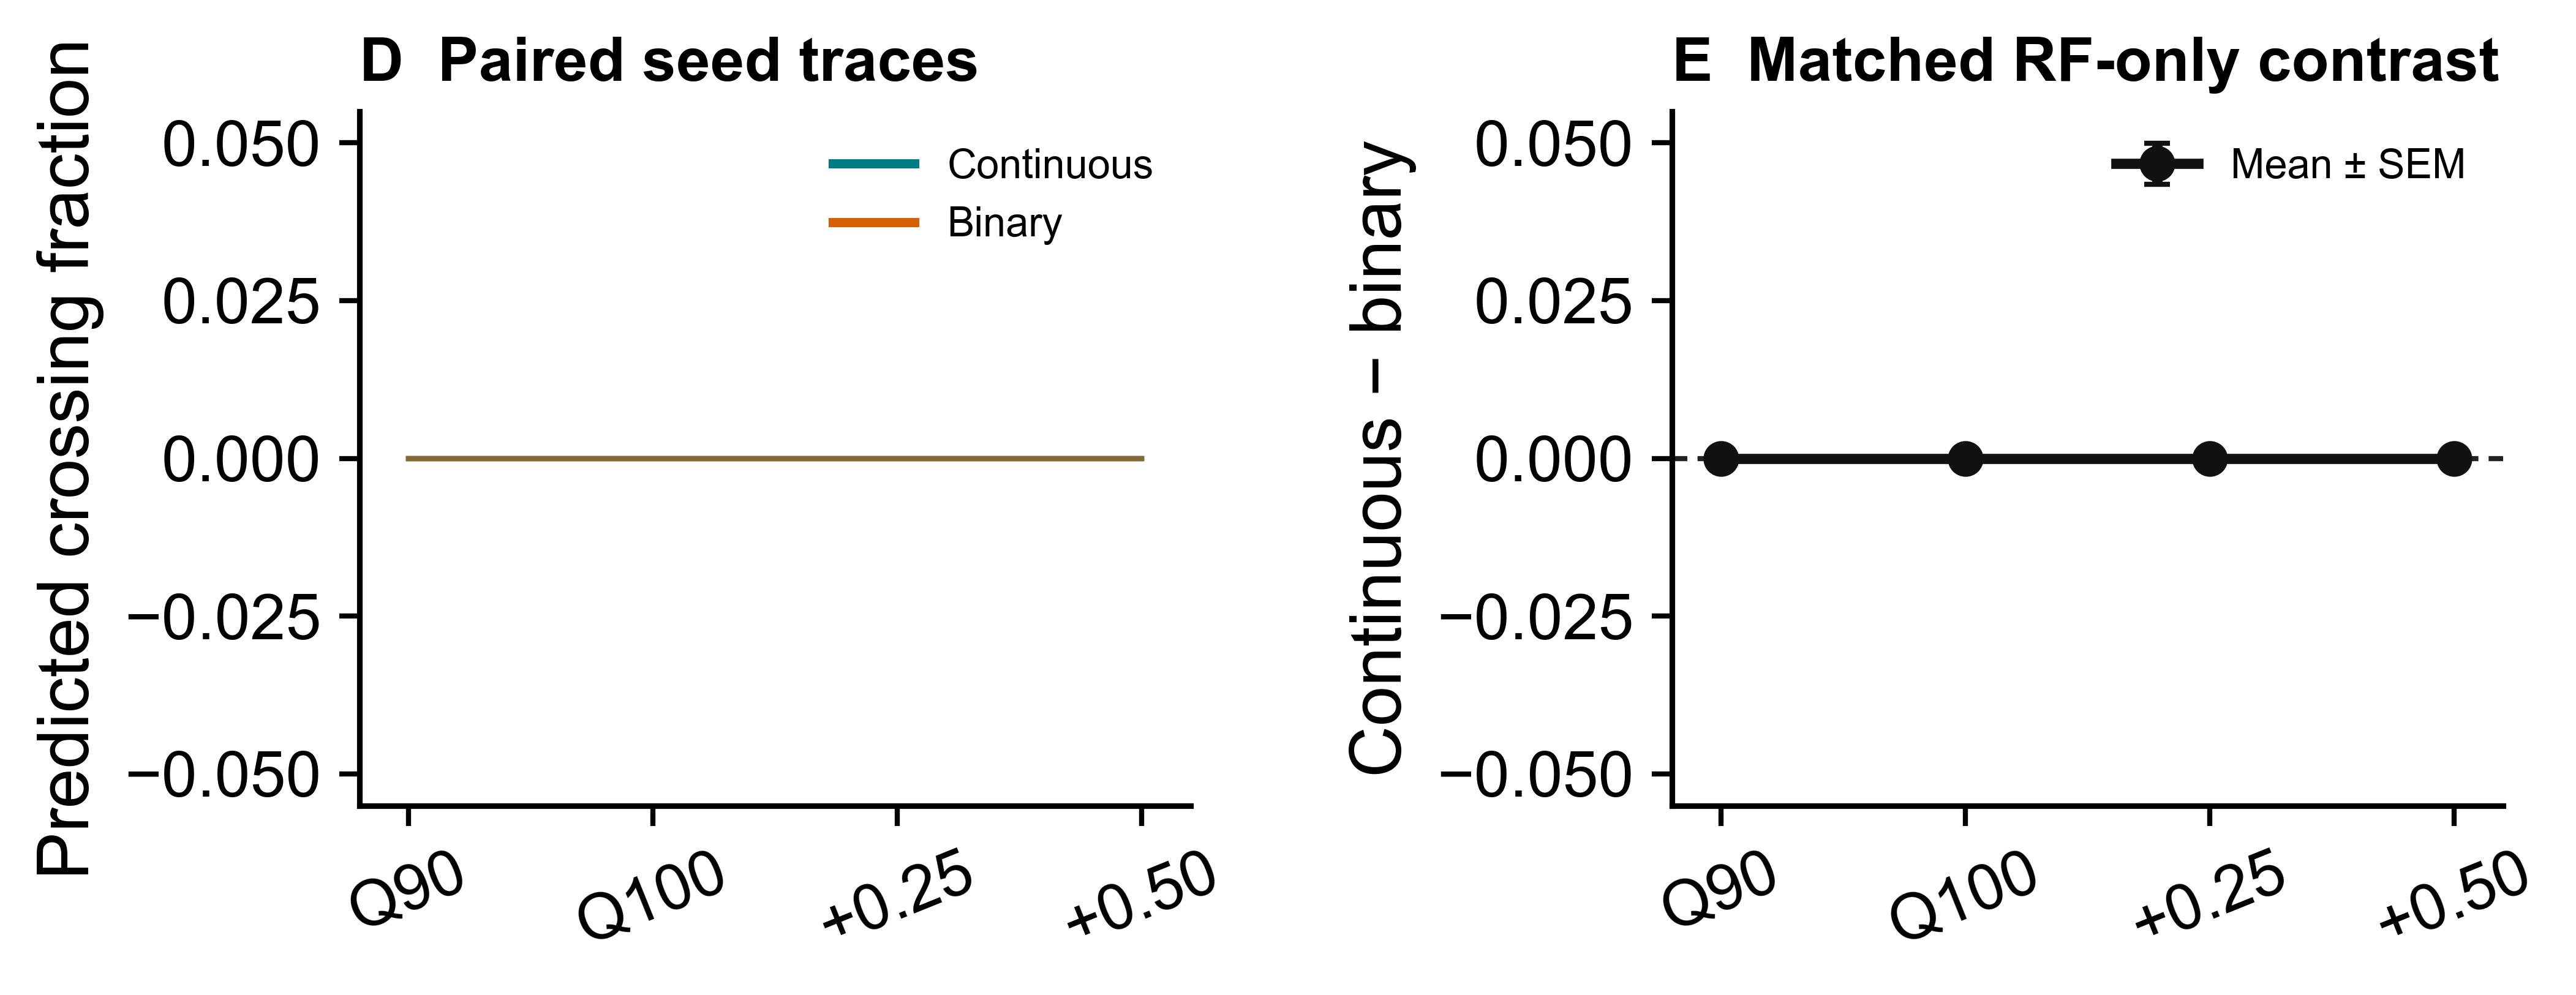
\includegraphics[width=0.98\linewidth]{figures/Figure_2_extrapolation_paired_contrast.png}
\caption{Paired extrapolation contrast across five seeds. Differences between conditioning arms do not change the zero frontier-crossing conclusion.}
\label{fig:extrapolation-contrast}
\end{figure}

This result is not evidence that the generator never produces high-scoring structures under any verifier. It is a narrower and stronger statement: under the frozen HTP-MD data source, representation and protocol, no arm generated a candidate that simultaneously satisfied the pre-registered validity/support/uncertainty gates and crossed the independently audited RF frontier. MD was not run by contract, so no physical or experimental extrapolation claim is made.
